\documentclass{article}

\usepackage{geometry}
\usepackage{makecell}
\usepackage{array}
\usepackage{multicol}
\usepackage{setspace}
\usepackage{changepage}
\usepackage{booktabs}
\usepackage{graphicx}
\usepackage{float}
\newcolumntype{?}{!{\vrule width 1pt}}
\renewcommand\theadalign{tl}
\newcommand{\paragraphlb}[1]{\paragraph{#1}\mbox{}\\}
\setstretch{1.10}
\setlength{\parindent}{0pt}

\geometry{top=12mm, left=1cm, right=2cm}
\title{Netzwerktechnologien Übung 2}
\author{Andreas Hofer}

\begin{document}
	\maketitle
	\section{MAC-Adressen}
	\begin{itemize}
		\item{Geben Sie ihre MAC-Adresse an:}
		\begin{itemize}
			\item{\verb|78:4F:43:A2:AA:9B|}
		\end{itemize}
		\item{Finden Sie heraus, welcher Hersteller mit ihrer MAC-Adresse assoziiert wird.}
		\begin{itemize}
			\item{\verb|78:4F:43|  ist eine OUI von Apple Inc.}
		\end{itemize}
		\item{Wandeln Sie ihre MAC-Adresse in Binärzahlen um.}
		\begin{itemize}
			\item{\verb|78:4F:43:A2:AA:9B|$_{16}$ in Hexadezimal ist \verb|0111 1000 0100 1111 0100 0011 1010 0010 1010 1010 1001 1011|$_2$ in Binär}
		\end{itemize}
	\end{itemize}
	\section{Analysieren von Ethernet Frames}
	\paragraphlb{Finde den ersten Ethernet-Frame/Paket und klicke darauf, um die Paketdetails anzusehen. Machen Sie einen Screenshot und markieren Sie die Ziel- und Sender-MAC Adresse.}
	\begin{figure}[H]
		\centering
		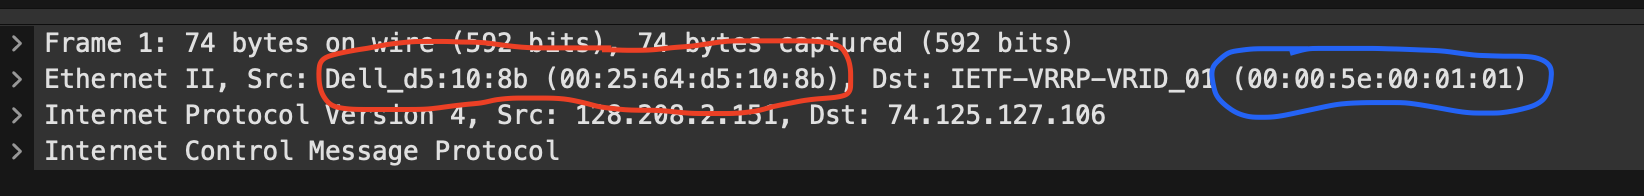
\includegraphics[scale=0.5]{Pictures/Capture1.png}
		\caption{Rot umrandet ist die Sender MAC-Adresse zusammen mit der Hersteller Adresse und blau umrandet die Empfänger MAC-Adresse.}
	\end{figure}
	\paragraphlb{Lassen Sie sich eines der Pakete anzeigen, dessen Protokoll als ARP gelistet ist. Machen Sie auch
	hier einen Screenshot und markieren Sie die Ziel- und Sender-MAC Adresse.}
	\begin{figure}[H]
		\centering
		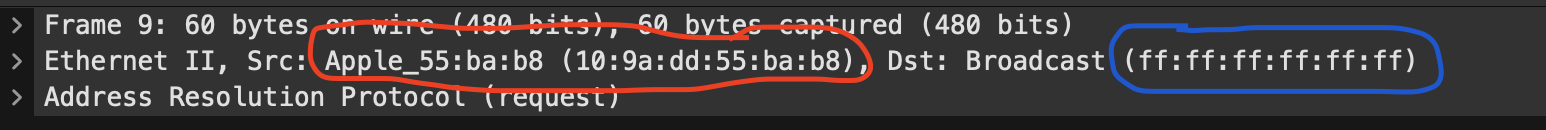
\includegraphics[scale=0.5]{Pictures/Capture2.png}
		\caption{Erneut in rot Sender MAC-Adresse und Hersteller und in blau Empfänger MAC-Adresse.}
	\end{figure}
	\paragraphlb{Was bedeutet die Ziel-MAC-Adresse: FF:FF:FF:FF:FF:FF:FF?}
	Es ist ein Broadcast. Da der Sender nicht weiß wo die Zieladresse liegt schickt er sie überall hin.
	\paragraphlb{Vergleichen Sie das Feld Type des ersten Paketes mit dem 12ten Paket. Beschreiben Sie in 1 bis 2 Sätzen, was dieser Unterschied bedeutet.}
	Die beiden Frames haben unterschiedliche Protokolle:
	\begin{itemize}
		\item{Internet Control Message Protocol (ICMP)}
		\begin{itemize}
			\item{Wird hier für einen Ping verwendet und dient wahrscheinlich für grundlegende Statusmitteilungen im Internet.}
		\end{itemize}
		\item{Address Resolution Protocol (ARP)}
		\begin{itemize}
			\item{Wird hier verwendet um die MAC Adresse einer IP Adresse zu finden. Da es Address Resolution im Namen hat, ist das wahrscheinlich sein Hauptnutzen.}
		\end{itemize}
	\end{itemize}
	\paragraphlb{Schauen Sie sich Paket 12 genauer an. Welche(r) Teile des Ethernet-Paketes, die wir in der Vorlesung besprochen haben, werden Ihnen nicht in Wireshark angezeigt.}
	Die Frame Check Sequence scheint nicht vorhanden zu sein. Ich nehme an, dass, gleich wie bei Switches, die NIC sie auswertet, bevor sie überhaupt angenommen wird und ein abgelehnter Frame gar nicht in Wireshark auftaucht.
	\paragraphlb{Recherchieren Sie was es mit IEEE 802.3 Paketen (Pakete 20 bis 22) auf sich hat. Was ist der Unterschied zu der Ethernet Version die wir in der Vorlesung besprochen haben? }
	Das Spanning Tree Protocol (STP) ist ein Standard der IEEE und nicht der IETF, was eventuell daran liegt, dass dieser primär zur Fehlervermeidung von Hardwareswitches und nicht dem Internet verwendet wird. Da die IETF ihn nicht in einem RFC veröffentlicht hat, wurde er auch nicht Teil des Ethernet II Standards sondern des IEEE-eigenen.
	\begin{figure}[H]
	\centering
	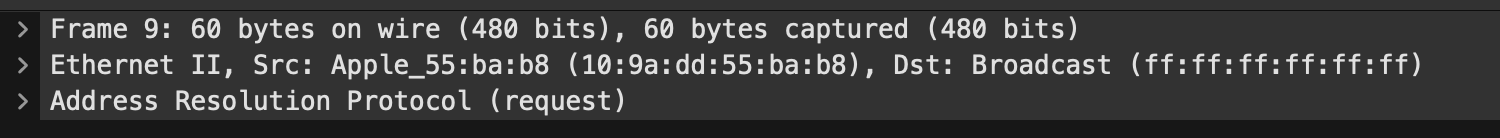
\includegraphics[scale=0.5]{Pictures/Capture3.png}
	\caption{Der Header des ARP Frames. Der Standard wird hier nur als Ethernet II angegeben}
	\end{figure}
	\begin{figure}[H]
	\centering
	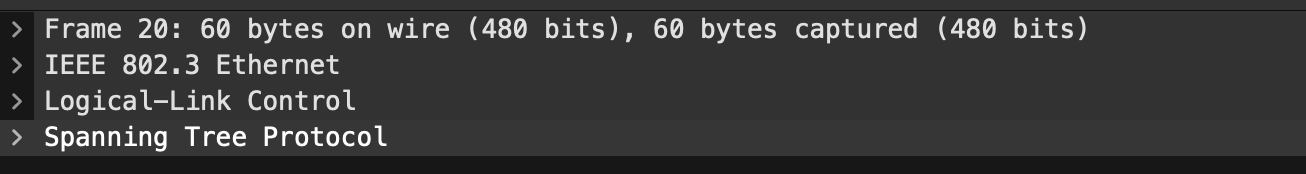
\includegraphics[scale=0.5]{Pictures/Capture4.png}
	\caption{Der Header des STP Frames. Der Standard wird hier hingegen als IEEE 802.3 Ethernet angegeben.}
	\end{figure}
	










	
\end{document}